\section{Systematics Evaluation}
\subsection{1 TS vs. 2 TS}
The very first systematic study that was performed is to compare the results between 2
firmware configurations. All of HF+ towers and half of HF- were sourced twice,
using either 1 TS (with Operating Voltage 1) or 2 TS (using Operating Voltage 2),
which provides us a measure of consistency in computing the calibration
coefficient across different firmware versions and operating voltages.
To compare these 2 modes of operation, we used ${CC}^{Run II}_{c}$ computed for
each sourcing configuration, after applying all the required corrections. The
distributions of ratios (1 TS over 2 TS) is presented in the figures~\ref{fig:HF_1TSto2TS}. Comparing 1 TS OV1 and 2 TS OV1+100 results, the source signals computed need to be corrected for the 25 ns vs 50 ns integration window. After correcting between the firmware gains, the results agree to an order of 1\%.

As observed in the Figures~\ref{fig:HF_1TSto2TS},
1 TS and 2 TS results match both for HF+ (1.4 \%) and HF- (0.3 \%) at the order of under 1.5 \%, which establishes solid indpendence of calibration coefficients from the firmware used.
\begin{figure}[htb]
  \centering
  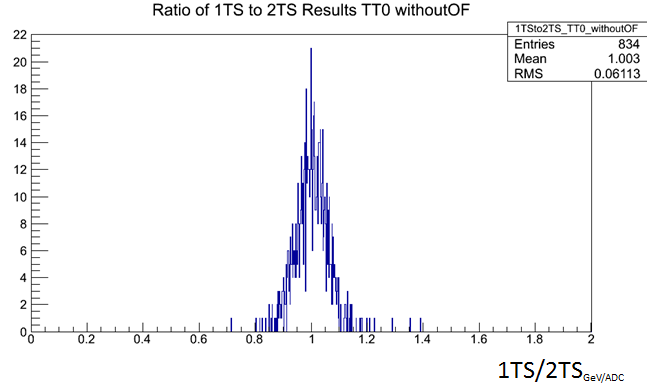
\includegraphics[width=0.45\linewidth]{figures/ch_hfcalibration/HFM_1TSto2TS_woOF.png}
  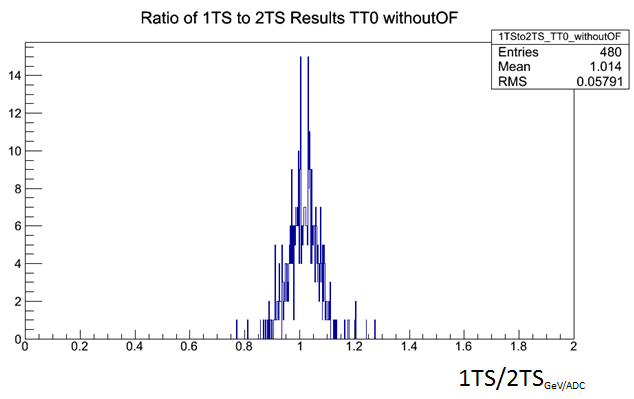
\includegraphics[width=0.45\linewidth]{figures/ch_hfcalibration/HFP_1TSto2TS_woOF.png}
  \caption
        {(a) Ratio of 1 TS/2 TS results for HF-.
         (b) Ratio of 1 TS/2 TS results for HF+
         For both sides The compared quantity was ${CC}^{Run II}_{c}$}
  \label{fig:HF_1TSto2TS}
\end{figure}
% \begin{figure}[!h]
%     \begin{center}
%         \subfigure[]
%         {
%             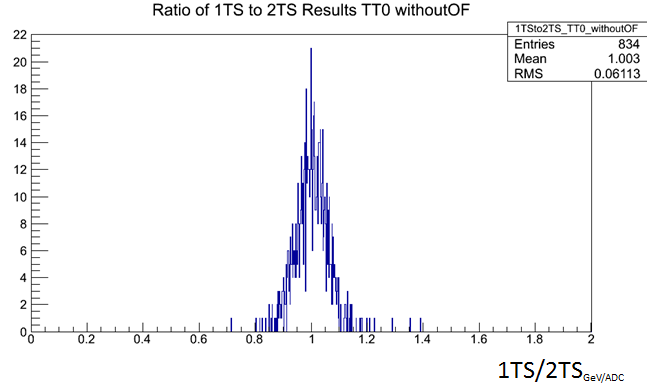
\includegraphics[width=.45\textwidth]{figures/ch_hfcalibration/HFM_1TSto2TS_woOF.png}
%         }\\
%         \subfigure[]
%         {
%             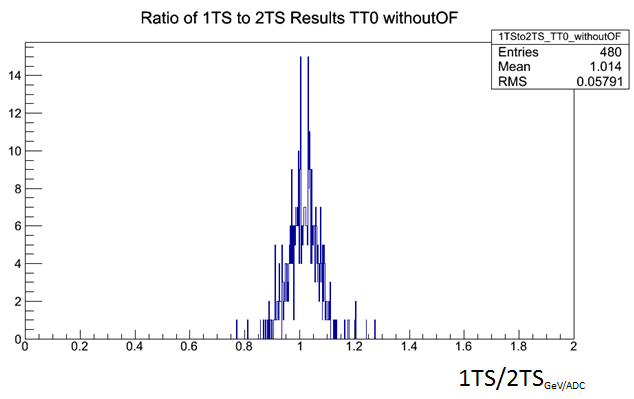
\includegraphics[width=.45\textwidth]{figures/ch_hfcalibration/HFP_1TSto2TS_woOF.png}
%         }
%     \end{center}
% \end{figure}

\subsection{Transversal Uniformity: Tubes A vs. Tubes B}
Approximately a quarter of HF wedges contains a second sourcing tube, which
differ in the groove type and as a consequence in the location within a wedge.
By comparing the obtained calibration coefficients using sourcing data from both
tubes, it is possible to extract information on the transversal uniformity of the signal within a wedge. Again, as in the case of 1 TS vs 2 TS study, the actual ${CC}^{Run II}_{c}$ are to be compared. The ratios are presented in figure \ref{fig:HF_A2B}. Transversal uniformity between A and B tubes within towers containing them show good agreement between results as well, differing by under 1\%.
\begin{figure}[htb]
    \centering
    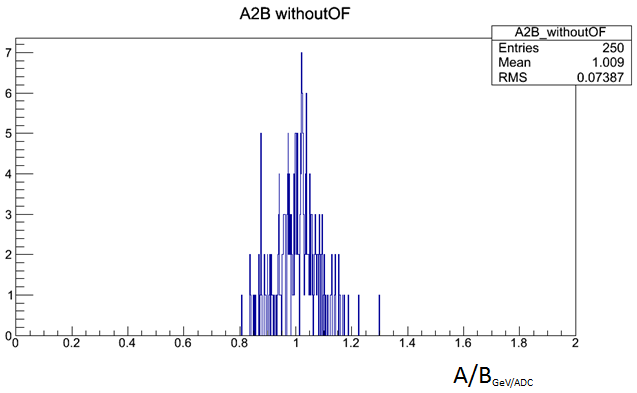
\includegraphics[width=.45\textwidth]{figures/ch_hfcalibration/HFM_A2B_woOF.png}
    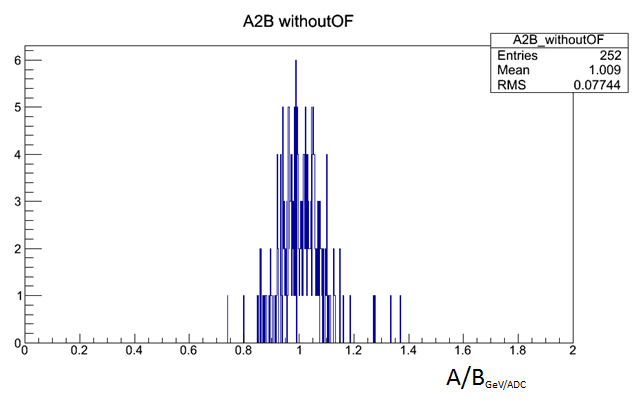
\includegraphics[width=.45\textwidth]{figures/ch_hfcalibration/HFP_A2B_woOF.png}
    \caption{(a) Ratio of A/B results for HF-. (b) Ratio of A/B results for HF+. For both sides the compared quantity was ${CC}^{Run II}_{c}$}
    \label{fig:HF_A2B}
\end{figure}

% \subsection{Overflow Estimation}
% Having the overflow bin is the major limitation of the DAQ system and the source of
% systematic uncertainty for our analysis. As it was mentioned in the Experimental
% Setup Section, both firmware types exhibit this behavior and even though 2TS
% has a wider ADC range, the results will not differ dramatically from 1TS, because
% differences in operating voltages will balance things out. However, in order to
% provide some kind of "Lower Bound" error estimation for our charge measurement,
% we separately computed calibration coefficients including the last bin in the
% Eq.~\ref{eq:Histo_Avg} and compared them to the ones computed without. The results
% for both HFM and HFP are presented in the Figure~\ref{fig:HF_Overflow}. Since we
% do not know the actual adc counts in the overflow, when computing charge, we used
% the center of the 32nd bin, as it was explained in the Experimental Setup section,
% using which does provide us with "Lower Bound" estimation.

% \begin{figure}[!h]
%     \begin{center}
%         \subfigure[]
%         {
%             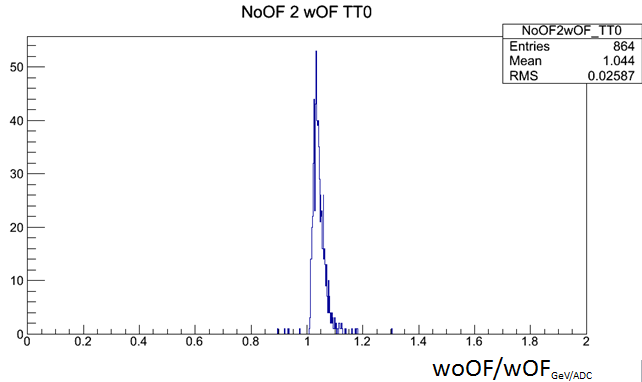
\includegraphics[width=.45\textwidth]{figures/ch_hfcalibration/HFM_NoOF2wOF_gevadc.png}
%         }~
%         \subfigure[]
%         {
%             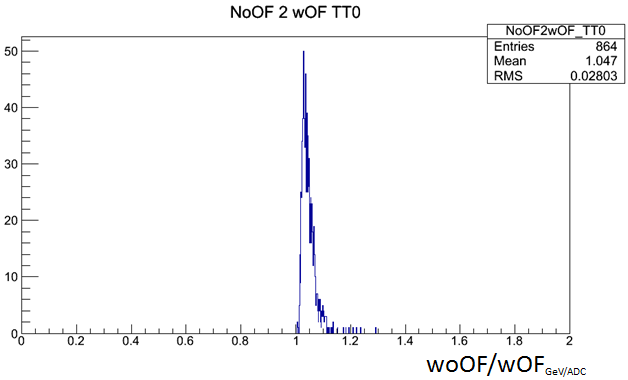
\includegraphics[width=.45\textwidth]{figures/ch_hfcalibration/HFP_NoOF2wOF_gevadc.png}
%         }
%         \caption
%         {(a) Ratio of woOF/wOF results for HFM.
%          (b) Ratio of woOF/wOF results for HFP
%          For both sides The compared quantity was ${CC}^{Run II}_{c}$.
%          Important to note that the ratio appears to be $\geq1$ because the compared quantity isn't a signal, but rather an actual calibration coefficient,
%          which contains energy over charge.}
%         \label{fig:HF_Overflow}
%     \end{center}
% \end{figure}

% As it can be observed in the Figure~\ref{fig:HF_Overflow}, the calibration
% coefficients computed including the overflow bin introduce at least 4.4-4.7\%
% difference into the measurement compared to the ${CC}^{Run II}_{c}$ computed
% excluding overflow. These 4.4-4.7\% give us a lower bound on the amount of charge
% that is approximately "sitting" in the overflow bin compared to the rest of the
% ADC range. However, taking into consideration that we subtracted the pedestal
% dynamically (inside the sum), we can notice that this is the amount of charge in
% the overflow compared to the actual charge deposited by the radioactive source
% (meaning that these charges are already pedestal-subtracted, which is very
% important, considering that number of events in the pedestal dominate substantially).
% Moreover, the actual number of events sitting in the overflow is under 1\% with
% respect to the same ADC range. And considering that our integration window is
% 25\unit{ns} long, it is important to exclude for calibration purposes any
% non-promptly originated signals.
% It is also important to note that overflow contribution was excluded when analyzing 2013 sourcin campaign, as it didn't contain just overflow charge, but it also any event which was marked as a "hardware failure" went into the overflow bin.

\subsection{Longitudinal Uniformity}
As the radioactive source is moving along the source tube, it is possible to actually record the spatial information on the location of the source, which provides with yet another tool to estimate the uncertainty of our measurements. The general idea is that several regions along the source tube are defined and histograms for each region respectively are summed up and then charged are extracted and compared.

As it was described in section \ref{section:experimentalsetup}, the tubes' start (tubeStart) and end (tubeEnd) positions are provided. In table~\ref{tab:TubeRegions} definitions of the tubes' regions of interest are formally defined. ''Front'' and ''Back'' are defined so that ''Front'' is closer to IP and ''Back'' is further away. ''Signal'' is the region that has been used as the defining region for extracting
the charge to be used in calibration coefficient calculation. And the ''$\frac{2}{3}$Back''
is an additional region defined to compare with the ''Signal''. It should be
noted that ''$\frac{2}{3}$Back'' and ''Signal'' have overlapping and non-overlapping
regions. Even though overlapping region is the dominant one, using these 2 regions it is possible to estimate how much the choice of the region influences the actual charge computed.
\begin{table}[!h]
    \centering
    \caption{Source tube regions defined to provide a measure of uncertainty on
    the charge deposited in various regions along the source tube}
    \begin{tabular}{|c|c|c|}
    \hline
    Region Name & Start & End \\
    \hline
    Front (Depth 1 or EM) & Tube End - 400 & Tube End-100 \\
    Front (Depth 2 or H) & Tube End - 700 & Tube End-400 \\
    Back & Tube Start+100 & Tube Start + 400 \\
    $\frac{2}{3}$ Back & Tube Start & Tube Start + $\frac{2}{3}$ (Tube End - Tube Start) \\
    Signal (EM and H) & Tube Start + 300 & Tube End-300 \\
    \hline
    \end{tabular}
    \label{tab:TubeRegions}
\end{table}

From figure \ref{fig:HF_LongUni}, observe that the signal in ''Front'' region is about 94 - 95 \% of the signal in the ''Back'' region. But it is neccessary to be more careful here when attributing this to systematics, as this mean ratio is consistent with the light attenuation in non-damaged fibers. Therefore, this 5 - 6 \% cannot be fully attributed to the systematic uncertainty. Considering the signal in ''$\frac{2}{3}$ Back'' with respect to the "Signal" region, a difference of 2\% on average is observed, which is the the contribution to the systematic uncertainty due to the longitudinal non-uniformity of the signal.
\begin{figure}[htb]
    \centering
    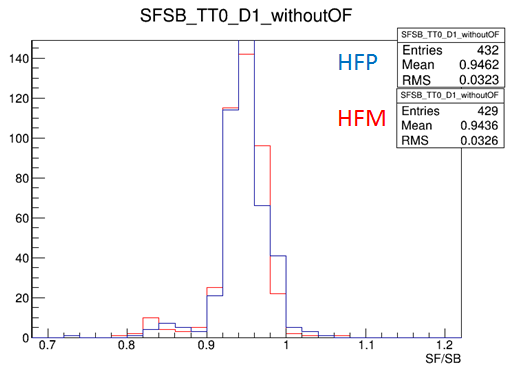
\includegraphics[width=.45\textwidth]{figures/ch_hfcalibration/SFSB_D1_woOF.png}
    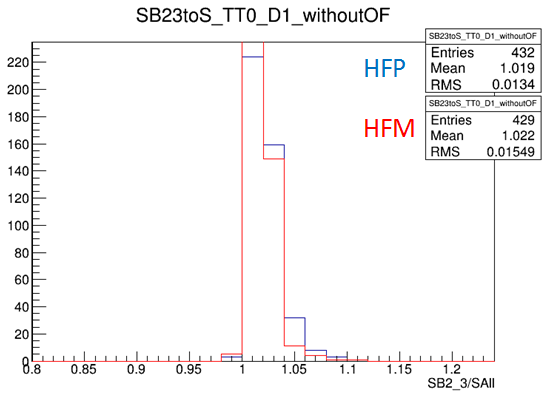
\includegraphics[width=.45\textwidth]{figures/ch_hfcalibration/SB23toS_D1_woOF.png}
    \caption{(a) Ratio of the charge extracted from the ''Front'' region to the charge computed in the region ''Back''. (b) Ratio of the charge computed within ''$\frac{2}{3}$ Back'' region to the ''Signal'' region. }
    \label{fig:HF_LongUni}
\end{figure}

\subsection{Cross Check}
An additional systematic uncertainty is included for the
methodology described in this note for measuring the absorber response to the source energy. Independent analyses were performed on the same data, and the results were compared and agree within an order of 1 \%, as it can be deduced from figure \ref{fig:Crosscheck}.
\begin{figure}[htb]
    \begin{center}
        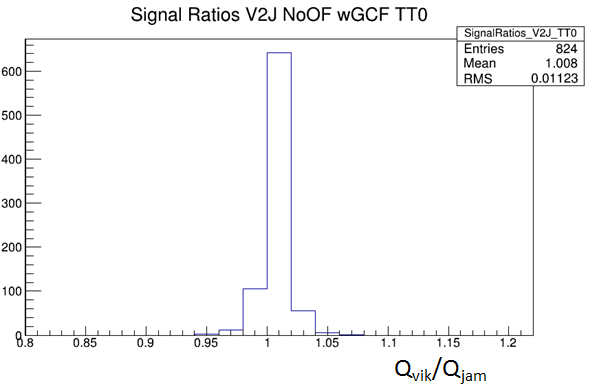
\includegraphics[width=.5\textwidth]{figures/ch_hfcalibration/Crosscheck.png}
        \caption{Cross-checking the results for HFM. On average the results agree
        within 1\%.}
        \label{fig:Crosscheck}
    \end{center}
\end{figure}